\documentclass[a4paper,12pt]{article}

% Packages
\usepackage[utf8]{inputenc}
\usepackage{amsmath, amssymb} % Math packages
\usepackage{graphicx} % For including images
\usepackage{hyperref} % For clickable links
\usepackage{geometry} % Page layout
\usepackage{subcaption} % For subfigures
\geometry{margin=1in}

% Title Page
\title{
    A Framework to Understanding the Implication of Automatically Reading the SMS by the Application on Smartphone.
    \vfill
    
\includegraphics[width=0.4\textwidth]{../images/iith_logo.png}
    \vfill
    }
\author{Jarpula Bhanu Prasad \\ 
\texttt{ai21btech11015@iith.ac.in} \\ 
\textit{Under the guidance of: Dr. Saurabh Kumar} \\ 
\texttt{saurabhkr@cse.iith.ac.in}}
\date{\today}

\begin{document}

\maketitle
\pagebreak

\begin{abstract}
    This project explores the implications of mobile applications that automatically read SMS messages, with a specific focus on OTPs (One-Time Passwords). The framework developed demonstrates the potential harm of such features by showcasing a simulated environment where messages are intercepted and analyzed. The system includes a broadcaster Android application to send received messages to a server, a Flask server for forwarding SMS to an Android emulator, and a rooted emulator with Firda-server installed for API hooking. By testing APIs of popular services, we proposes this framework for future security testing and awareness regarding the misuse of automatic OTP readers.
\end{abstract}

\vfill

\tableofcontents

\vfill

\section*{Acknowledgement}
I would like to express my deepest gratitude to my advisor, Dr. Saurabh Kumar, for their invaluable guidance, encouragement, and support throughout the course of this project. Their insightful feedback and expertise were instrumental in shaping the direction and execution of this work. I am profoundly thankful for the time and effort they dedicated to mentoring me, which greatly enhanced my learning experience.

Their patience and belief in my abilities have been a source of constant motivation, and I am truly fortunate to have had the opportunity to work under their guidance.
\pagebreak

\section{Introduction}
With the increasing reliance on SMS-based authentication, mobile applications often include features to automatically read SMS messages containing OTPs for seamless user experience. However, these features introduce significant security and privacy risks if exploited maliciously. Unauthorized access to OTPs can compromise sensitive accounts and bypass two-factor authentication mechanisms.

This project aims to investigate the potential harm caused by automatic OTP readers in mobile applications. A comprehensive framework has been developed to simulate and analyze the vulnerabilities in such systems. The framework includes:

\begin{enumerate}
    \item A rooted Android emulator equipped with Firda-server for deeper analysis, enabling the hooking of APIs from popular services.
    \item A broadcaster Android application that captures and sends received messages to a destination server.
    \item A Flask-based Python server that forwards SMS data from Android devices to a rooted Android emulator running on the server.
\end{enumerate}

\begin{figure}[h]
    \centering
    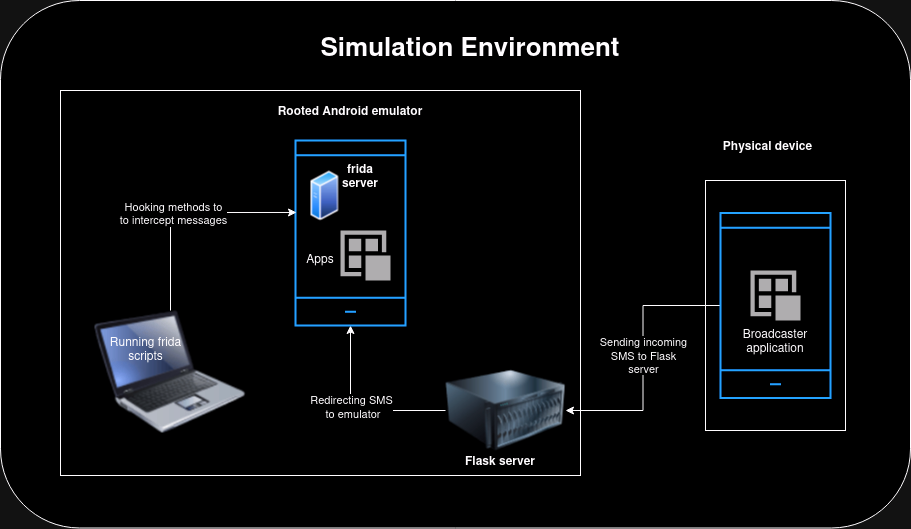
\includegraphics[width=0.9\textwidth]{../images/architecture.png}
    \caption{Framework Overview}
\end{figure}
By utilizing this setup, the framework demonstrates the risks of unauthorized OTP interception and manipulation, offering a tool for future security research and application testing. This project underscores the need for stricter safeguards in mobile applications to mitigate these risks and protect user data.

\section{Methodology}
\subsection{Rooting the Android Emulator}
\subsubsection{Why Use an Emulator Instead of a Physical Device?}

Using an Android emulator rather than a physical device for experimentation offers several advantages, particularly in projects involving rooting or API hooking:

\begin{enumerate}
    \item \textbf{Cost-Effectiveness}:Emulators are free and readily available through tools like Android Studio. In contrast, physical devices can be expensive, especially if multiple devices are required for testing.
    \item \textbf{Risk Mitigation}: Rooting a physical device involves risks such as bricking the device due to errors during the process. This can render the device unusable, leading to significant costs and downtime.
    \item \textbf{Convenience}:Emulators provide a controlled and repeatable environment for testing. They allow for easy snapshots and resets, enabling developers to experiment without the fear of permanent damage.
    \item \textbf{Accessibility of Features}:Tools like Magisk or Firda-server can be installed on emulators with fewer restrictions, making it easier to simulate complex use cases like OTP interception or API hooking.
\end{enumerate}

\subsubsection{Rooting an Android Virtual Device (AVD)}
Rooting an Android Emulator (AVD) involves modifying its system image to gain root access, enabling deeper customization and testing of applications. This process is useful for tasks such as API hooking and testing applications with elevated permissions. Below are the key steps to root an AVD:

\begin{enumerate}
    \item \textbf{Clone rootAVD Repository}:
    \begin{verbatim}
        $ git clone https://github.com/newbit1/rootAVD.git
    \end{verbatim}

    \item \textbf{Start avd agent}:
    \begin{verbatim}
        $ cd rootAVD
        $ ./rootAVD.sh
    \end{verbatim}

    \item \textbf{Start emulator and root}:
    \begin{verbatim}
     $ ./rootAVD.sh system-images/android-{<api-level>}/
     google_apis_playstore/<arch>/ramdisk.img
    \end{verbatim}

\end{enumerate}

\subsection{Developing the Broadcaster Android Application}
For the project, a broadcaster Android application was developed using the Flutter framework to handle SMS interception and communication with a designated server. Flutter was chosen due to its cross-platform capabilities, allowing for rapid development of an Android application with consistent performance and user experience across devices. Here's a breakdown of the key features and functionality of the application:
\begin{enumerate}
    \item \textbf{User Input for Server Details}: The application prompts the user to input the server's IP address and port number. These details are necessary to establish a connection between the mobile device and the server. The app saves this information for subsequent use.
    \item \textbf{SMS Message Interception}: Whenever the mobile device receives an SMS, the broadcaster application automatically reads the message using Android's SMS APIs. The app monitors incoming SMS messages, extracts the content, and prepares it for forwarding to the designated server.
    \item \textbf{Redirection to the Server}:Once the SMS is intercepted, the application establishes a connection with the pre-configured server and sends the message content. The communication between the mobile device and server is handled using standard protocols like HTTP or TCP, depending on the configuration set by the user. This allows for real-time forwarding of SMS data, making it useful for scenarios such as OTP forwarding or message logging.
    \item \textbf{Implementation in Flutter}:Flutter enables the use of native Android APIs, which is essential for accessing SMS and network communication features. For instance, the sms package in Flutter is utilized to listen for incoming messages, while the http package or socket communication is used to send the data to the server.
\end{enumerate}
This broadcaster application plays a crucial role in the broader context of the project by acting as the first step in the SMS interception chain. It allows the server to receive and process messages for further analysis or forwarding to other systems, making it an integral component of the framework designed to test the vulnerabilities of automatic OTP readers.

By using Flutter, the development process was streamlined, and the application was able to run on different devices with minimal additional coding, highlighting the benefits of cross-platform development for mobile applications

\subsection{Setting Up the Flask Server}
The Flask server in this project is responsible for handling HTTP requests from the broadcaster application, processing the received data, and forwarding it to the Android emulator via a Telnet connection. The server leverages the Flask framework to create a simple yet efficient HTTP interface for communication. Here's an explanation of its components and functionality:

\begin{figure}[h]
    \centering
    \begin{subfigure}[b]{0.75\textwidth}
        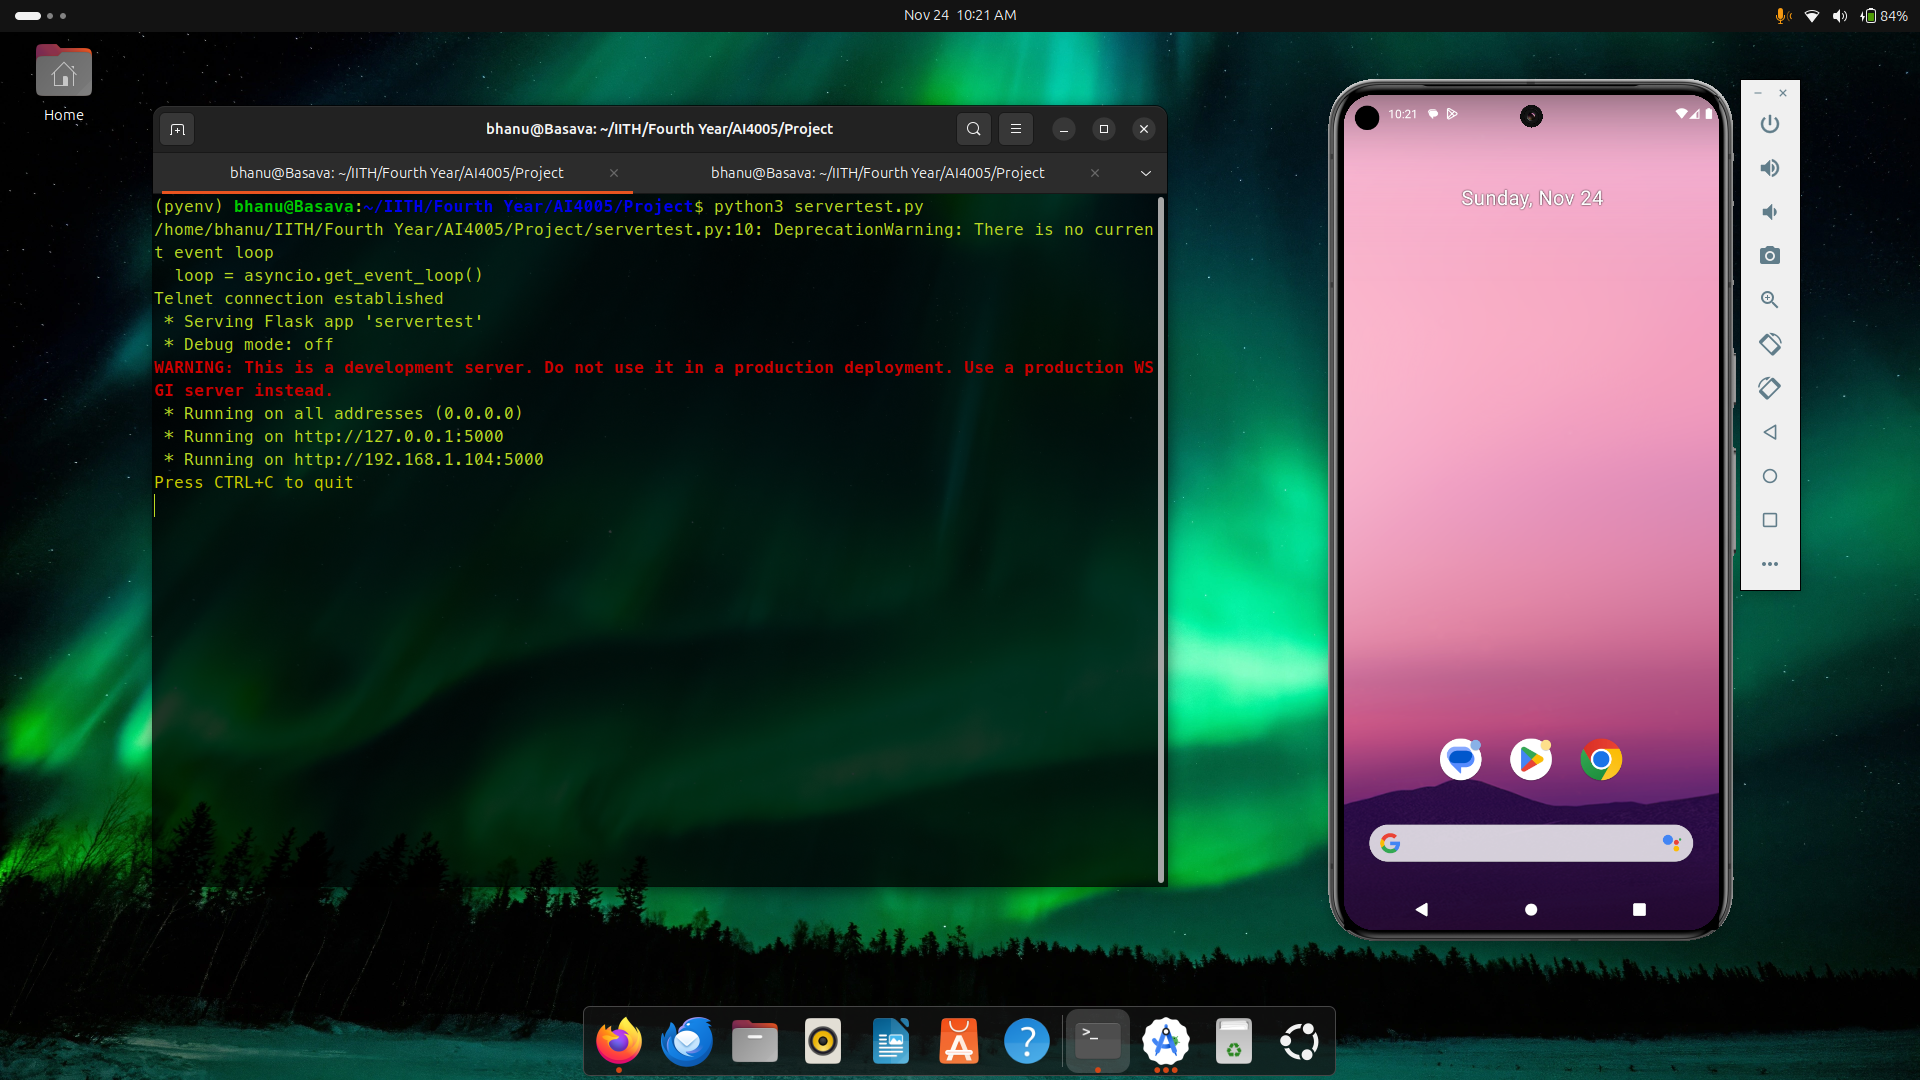
\includegraphics[width=\textwidth]{../images/python-sms-server.png}
        \caption{Setted flask server to receive application and forward to emulator}
    \end{subfigure}
    \hfill
    \begin{subfigure}[b]{0.2\textwidth}
        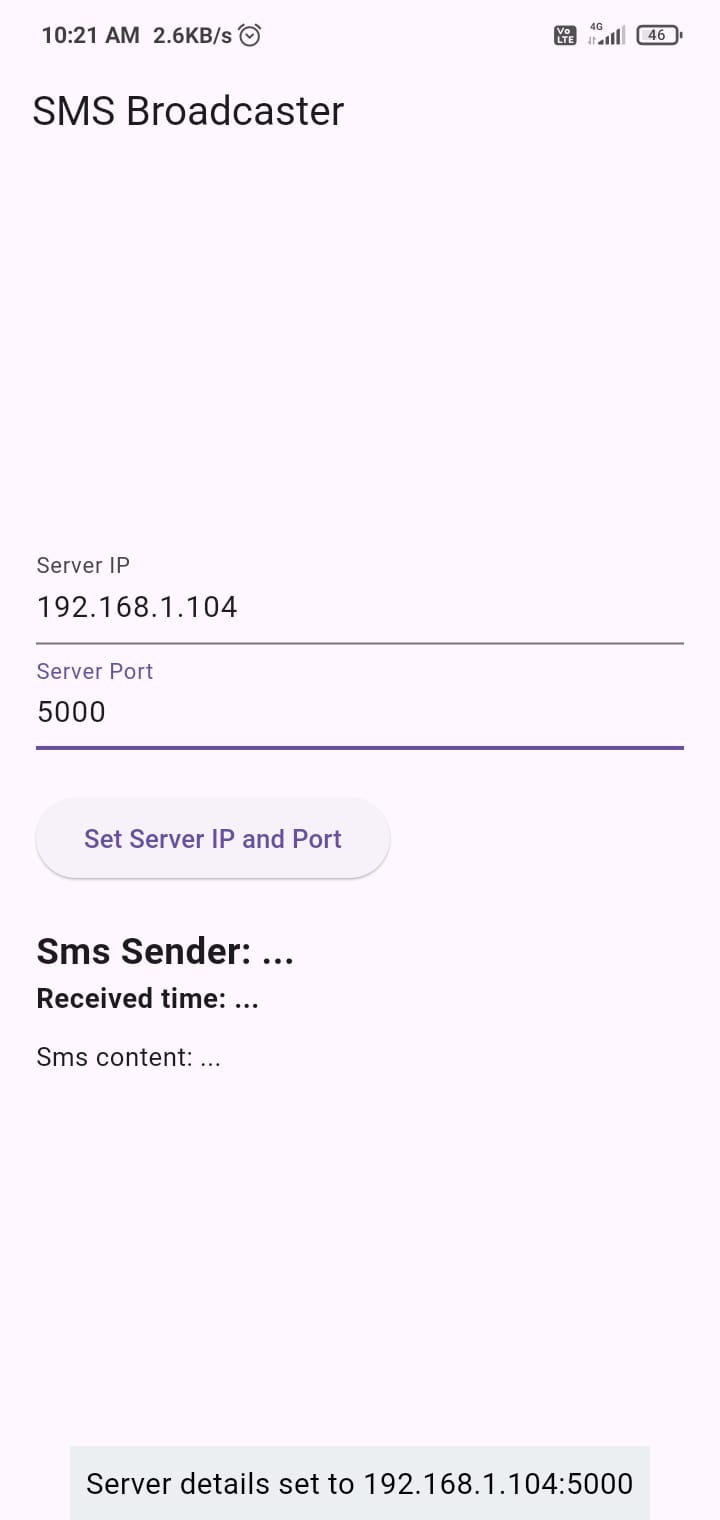
\includegraphics[width=\textwidth]{../images/setting-server-details.jpeg}
        \caption{broadcaster}
    \end{subfigure}
    \caption{Establishing communication between broadcaster and emulator}
\end{figure}

\begin{enumerate}
    \item \textbf{Flask Server Setup}: The server is initialized using the Flask framework, which listens for incoming POST requests at the root endpoint (/). These requests contain the SMS data received by the broadcaster Android app. Flask handles these requests and processes the JSON data sent by the mobile application.
    \item \textbf{Telnet Connection to Emulator}:The server establishes a Telnet connection to the Android emulator running on the server. This is done using the telnetlib3 package in Python, which allows asynchronous communication over Telnet. The server first authenticates with the emulator using an ADB authentication token, ensuring that it has permission to interact with the emulator.
    \item \textbf{Receiving and Forwarding SMS Data}:When the Flask server receives a POST request, it extracts the sender's phone number and the SMS message from the JSON payload. The server then formats this data into a Telnet command (sms send {sender} {message}) and sends it to the emulator via the established Telnet connection. This command triggers the emulator to simulate the SMS being received on the device.
    \item \textbf{Error Handling and Response}: The server includes error handling to ensure that if anything goes wrong during the Telnet communication, it responds with an error message. If the SMS data is successfully sent to the emulator, the server returns a success message.
    \item \textbf{Synchronization and Asynchronous Operations}: The server uses Python's asyncio to manage asynchronous operations. This is particularly useful for the Telnet connection, as it allows non-blocking communication with the emulator. The server uses synchronous wrappers to execute the asynchronous functions in a straightforward manner when interacting with Flask.
    \item \textbf{Running the Server}: Finally, the server is run on the host machine at port 5000, allowing it to accept incoming HTTP requests from the broadcaster application.
\end{enumerate}

\begin{figure}[h]
    \centering
    \begin{subfigure}[b]{0.75\textwidth}
        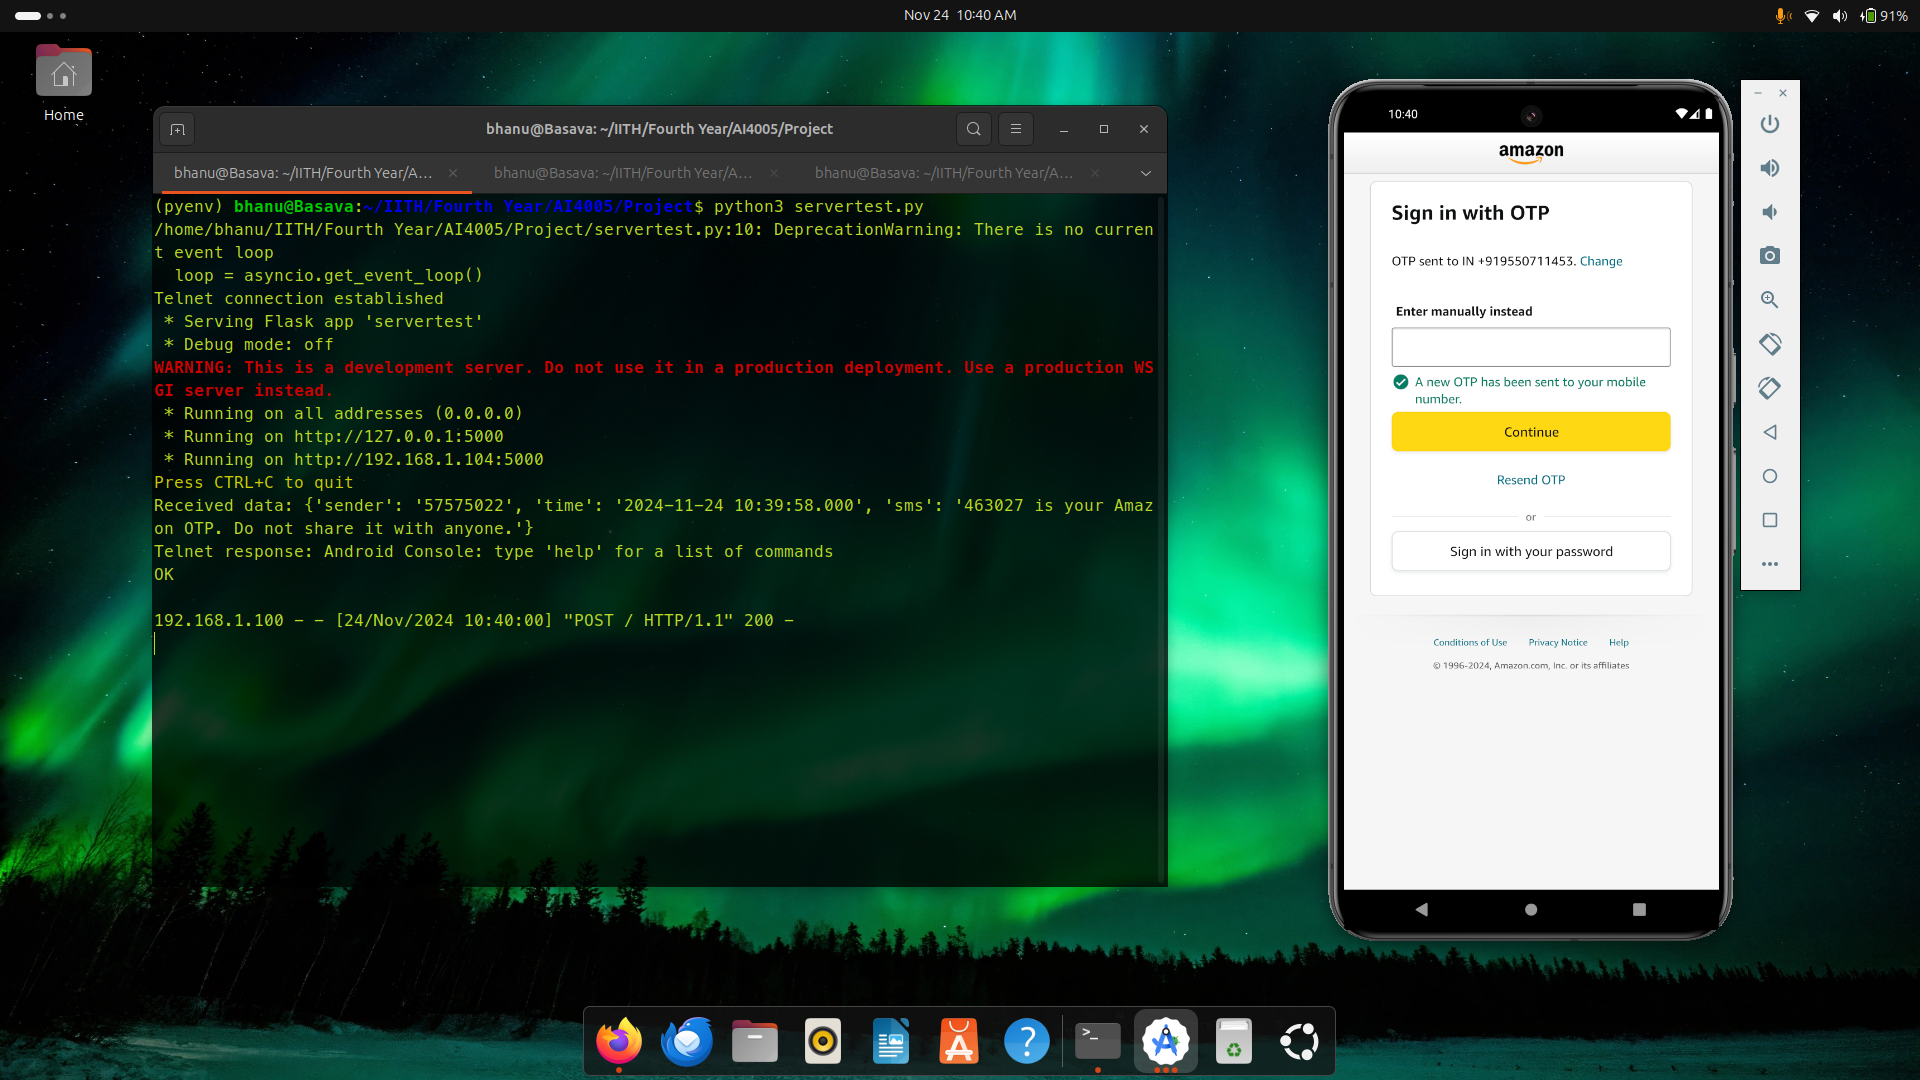
\includegraphics[width=\textwidth]{../images/sms-received-demo.png}
        \caption{Setted flask server to receive application and forward to emulator}
    \end{subfigure}
    \hfill
    \begin{subfigure}[b]{0.2\textwidth}
        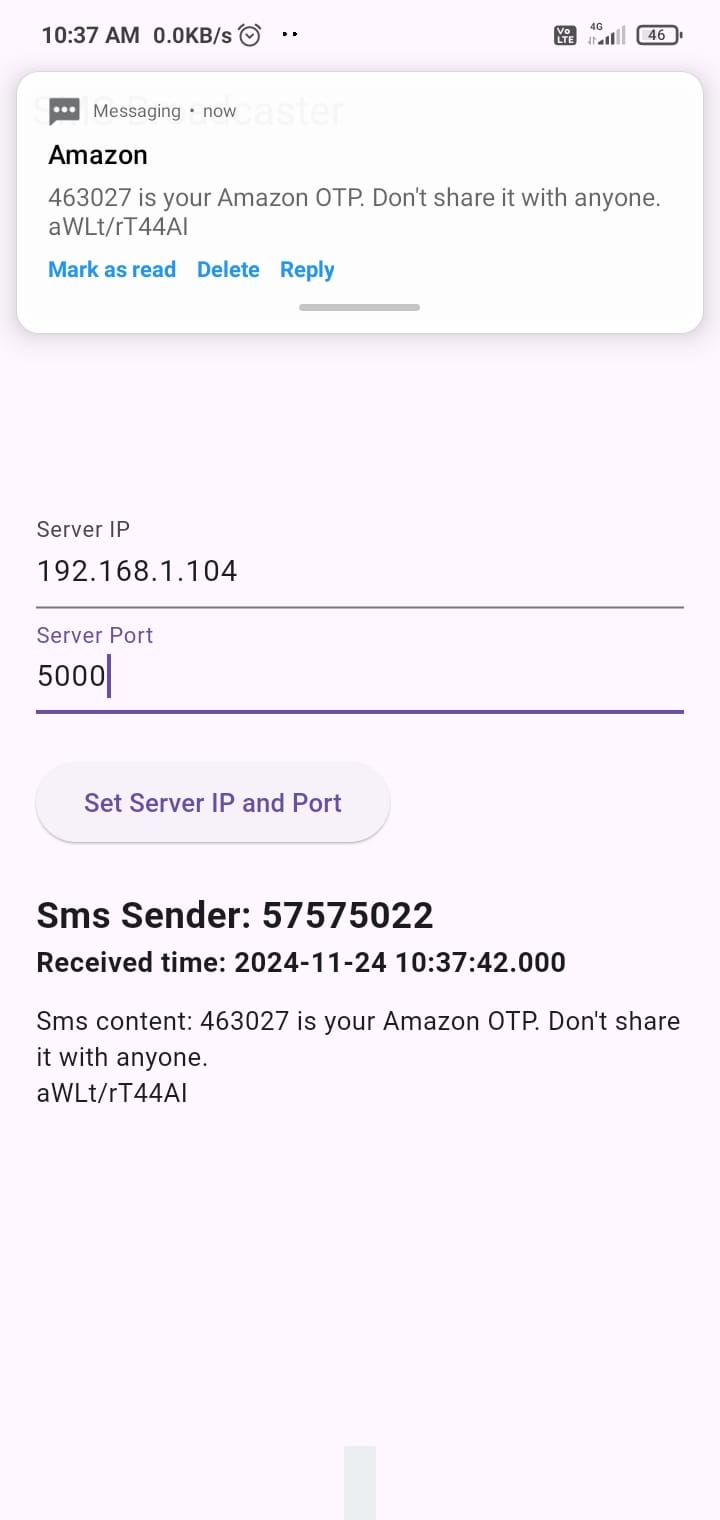
\includegraphics[width=\textwidth]{../images/sms-sent-demo.jpeg}
        \caption{broadcaster}
    \end{subfigure}
    \caption{Sending SMS from broadcaster to emulator via Flask server}
\end{figure}

By using this Flask server setup, the project establishes a communication channel between the broadcaster Android app and the emulator, enabling the forwarding of SMS messages for further testing and analysis.

\subsection{API Hooking with Frida-Server}
To enable API hooking and dynamic instrumentation of Android applications, we use Frida-server. Frida allows us to intercept and modify function calls in real-time, which is critical for analyzing the behavior of applications, especially for tasks like monitoring how they handle sensitive data such as OTPs. Below are the steps to install and configure Frida-server on a rooted Android emulator.

\begin{figure}
    \centering
    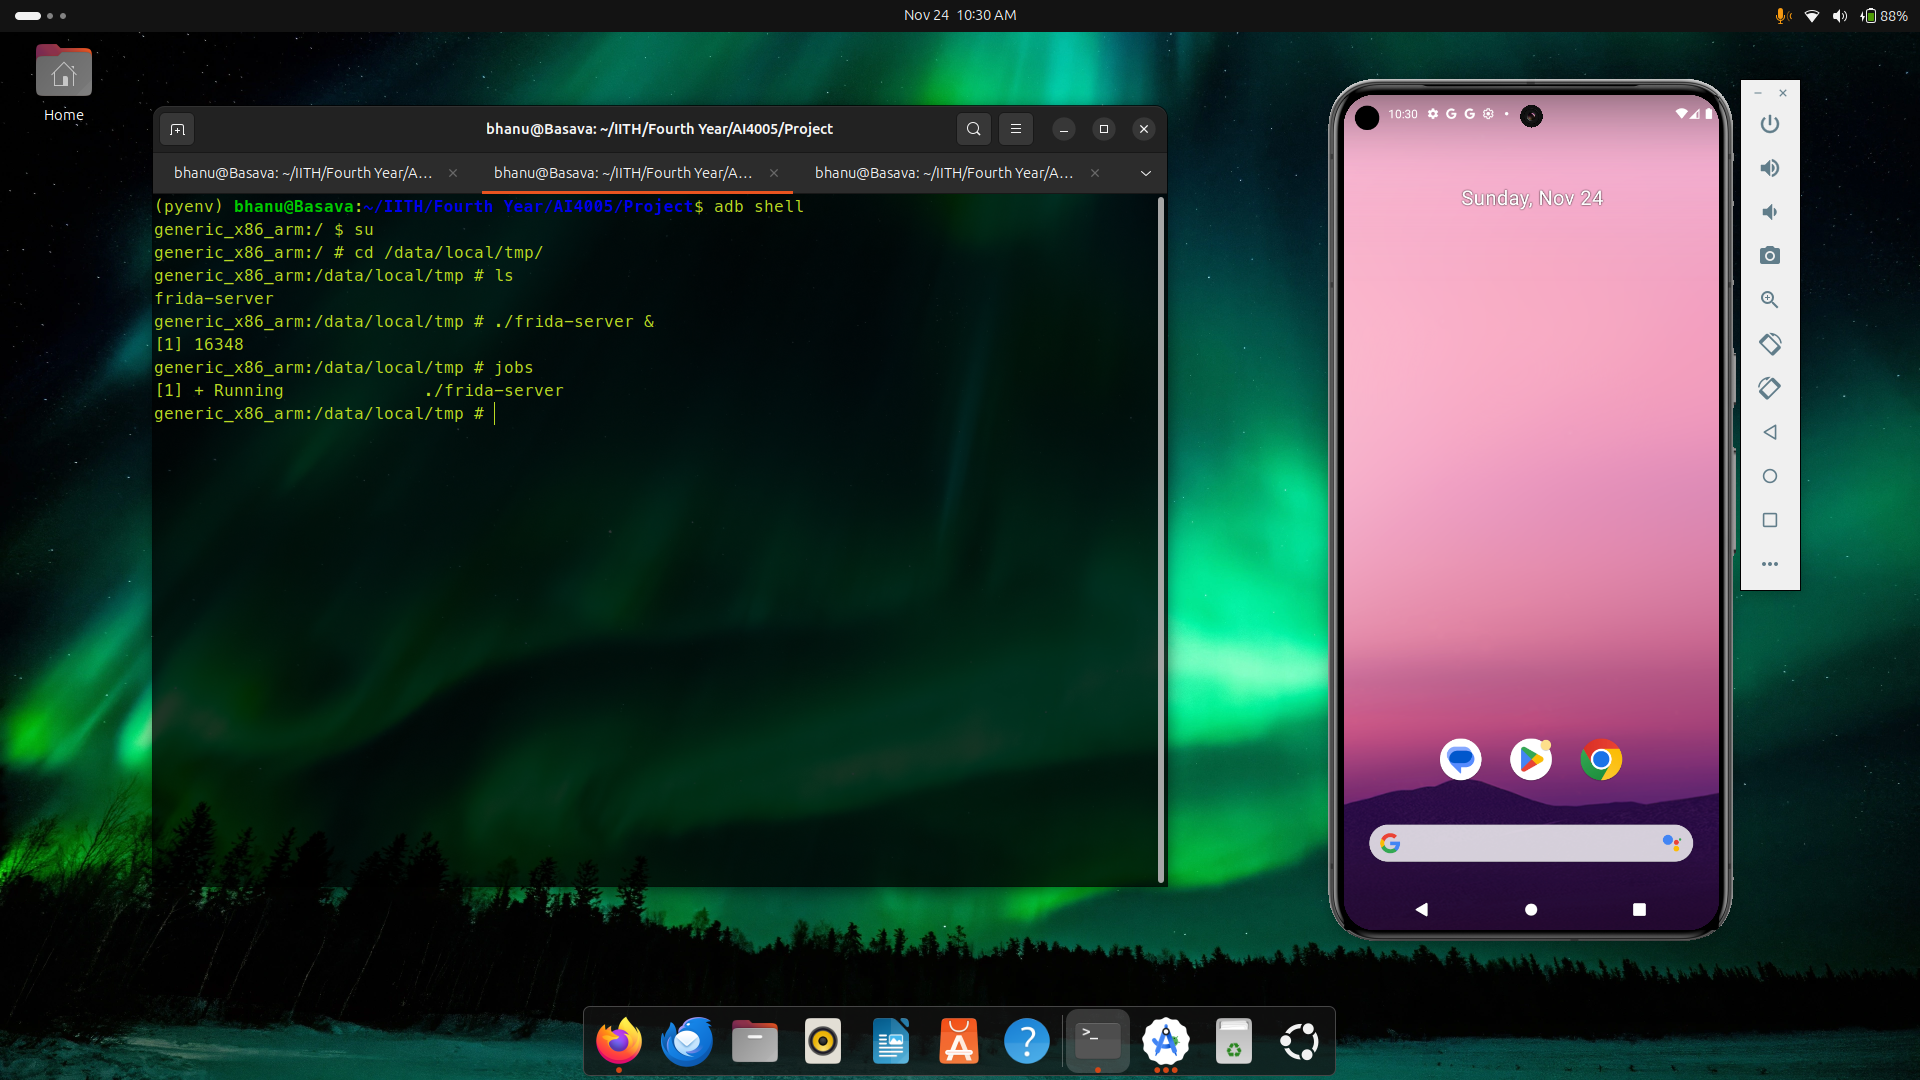
\includegraphics[width=0.9\textwidth]{../images/running-frida-on-emulator.png}
    \caption{Frida-server for API hooking}
\end{figure}
\begin{enumerate}
    \item \textbf{Copy Frida-Server to the Emulator}: First, you need to copy the Frida-server binary from your host system to the Android emulator using the adb push command.
    \begin{verbatim}
        $ adb push frida-server /data/local/tmp
    \end{verbatim}
    This command places the frida-server binary in the /data/local/tmp directory on the emulator, where it can be executed.
    \item \textbf{Set Appropriate Permissions} : Once the binary is copied, you need to grant it the necessary permissions to make it executable. This can be done using the chmod command inside the emulator.
    \begin{verbatim}
        $ adb shell "su -c chmod 755 /data/local/tmp/frida-server"
    \end{verbatim}
    \item \textbf{Start Frida-Server on the Emulator} : Now that the Frida-server binary is in place and properly configured, you can start it on the emulator. Since the emulator is rooted, you can run Frida-server with root privileges using the following command:
    \begin{verbatim}
        $ adb shell 'su -c "/data/local/tmp/frida-server" &'
    \end{verbatim}
    \item \textbf{Using Frida-Scripts to Monitor and Modify Application Behavior}: Once Frida-server is running, you can use Frida scripts to hook into specific functions or APIs of interest. Frida scripts are typically written in JavaScript and can be used to monitor and manipulate the behavior of applications in real time.
    \begin{verbatim}
        $ frida -U -f <package-name> -l <script-name>.js
    \end{verbatim}
\end{enumerate}

\begin{figure}[h]
    \centering
    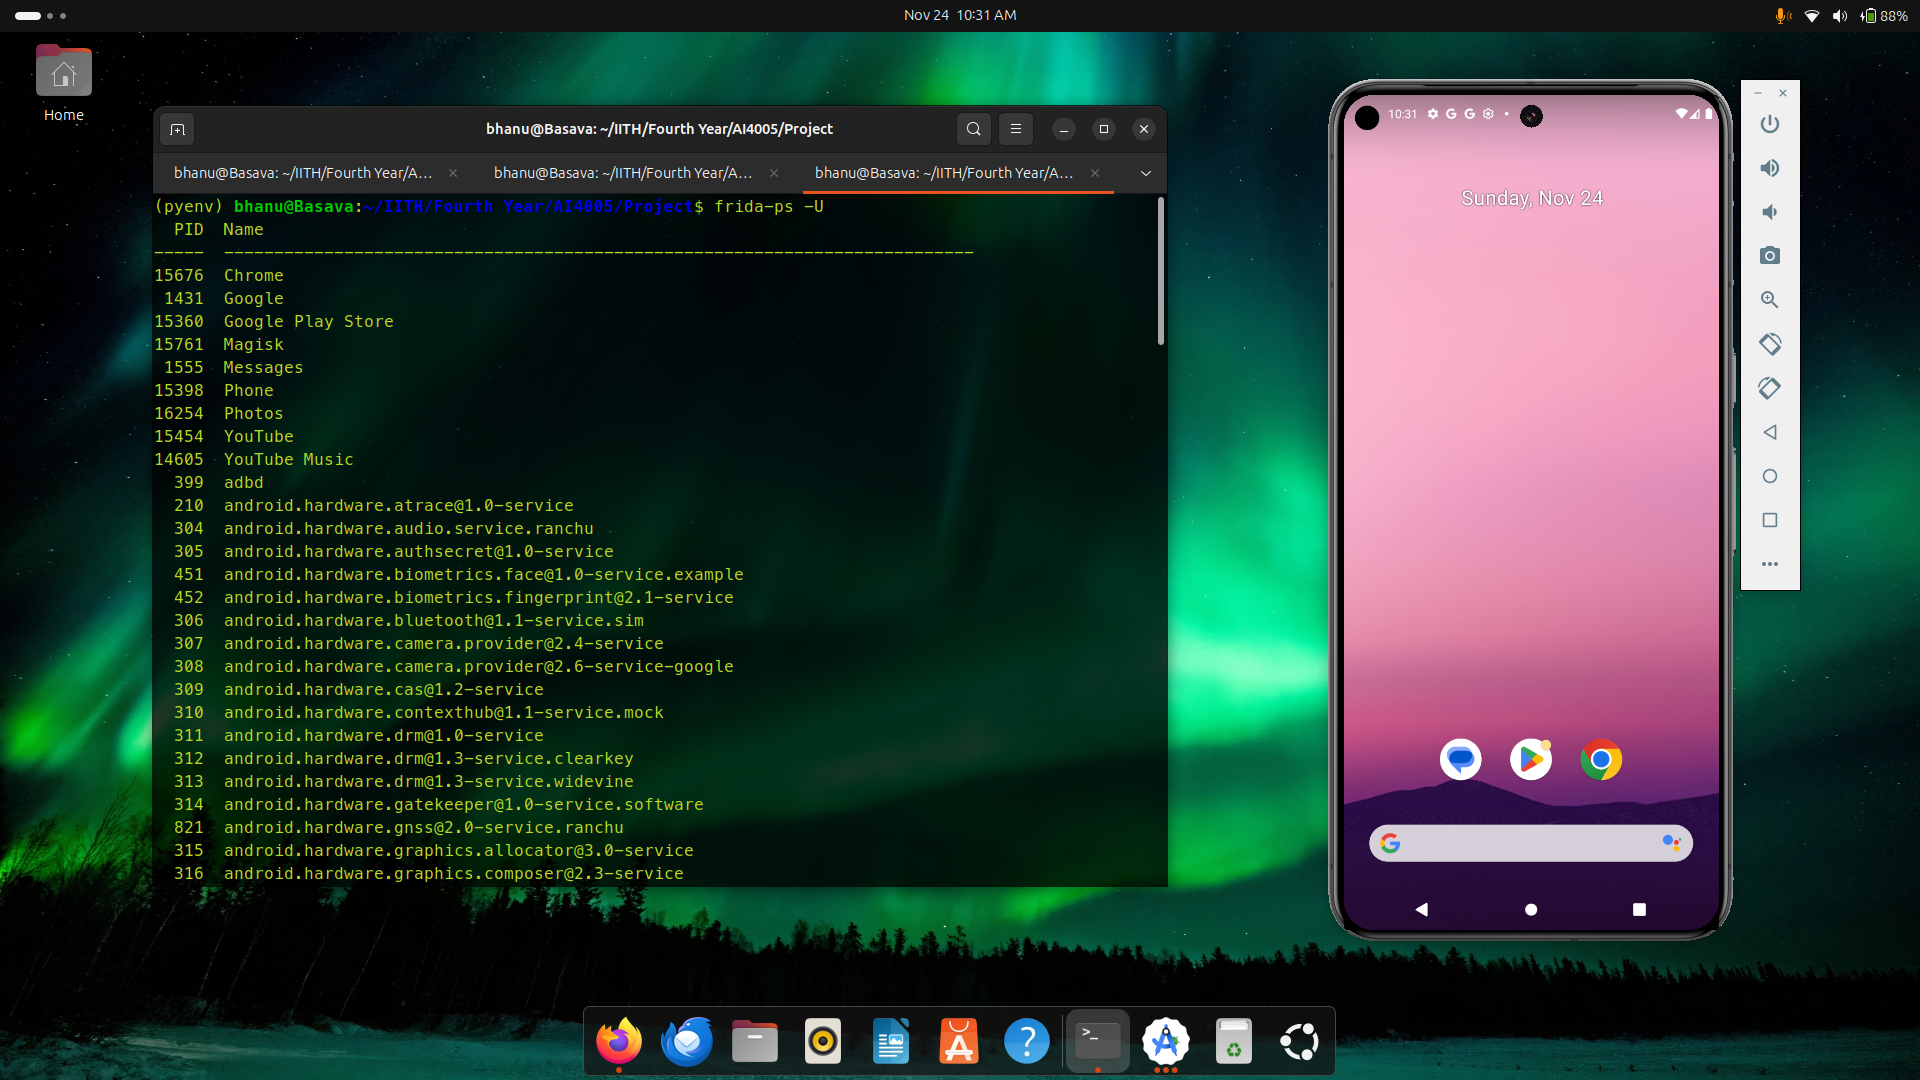
\includegraphics[width=0.9\textwidth]{../images/verifying-frida-running.png}
    \caption{Verifying Frida-server running on the emulator}
\end{figure}

\section{Discussion}
In jsFrida scripts \texttt{activity\_monitor.js} will list down all the activities that a mobile application using from here identify the activity that is responsible for reading the SMS.
\begin{figure}[h]
    \centering
    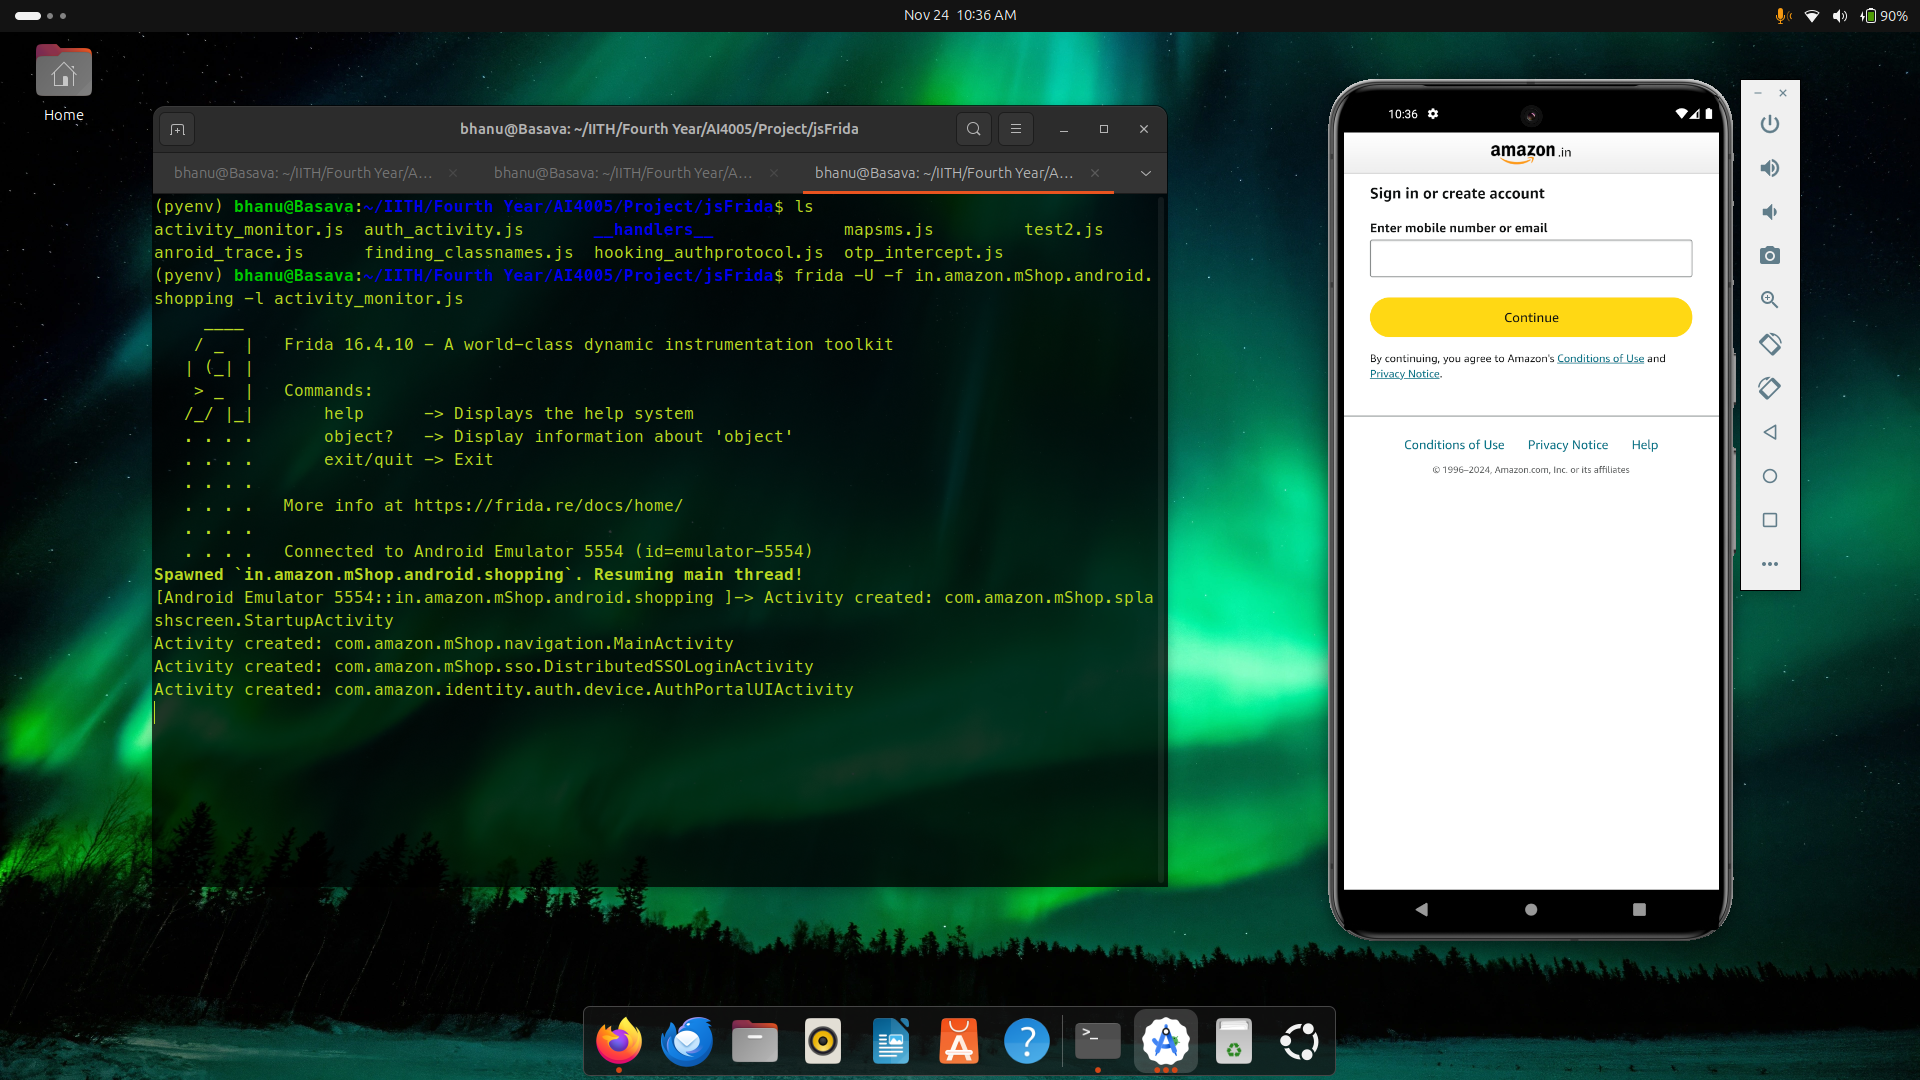
\includegraphics[width=0.9\textwidth]{../images/activity-monitor.png}
    \caption{Activity monitor using Frida}
\end{figure}

In above figure we see \texttt{com.amazon.identity.auth.device.AuthProtocolUIActivity} is responsible for reading the SMS. This activity is responsible for reading the OTP from the SMS and automatically filling it in the application.

lets hook into this activity and see the SMS that is being read by the application.
\begin{figure}[h]
    \centering
    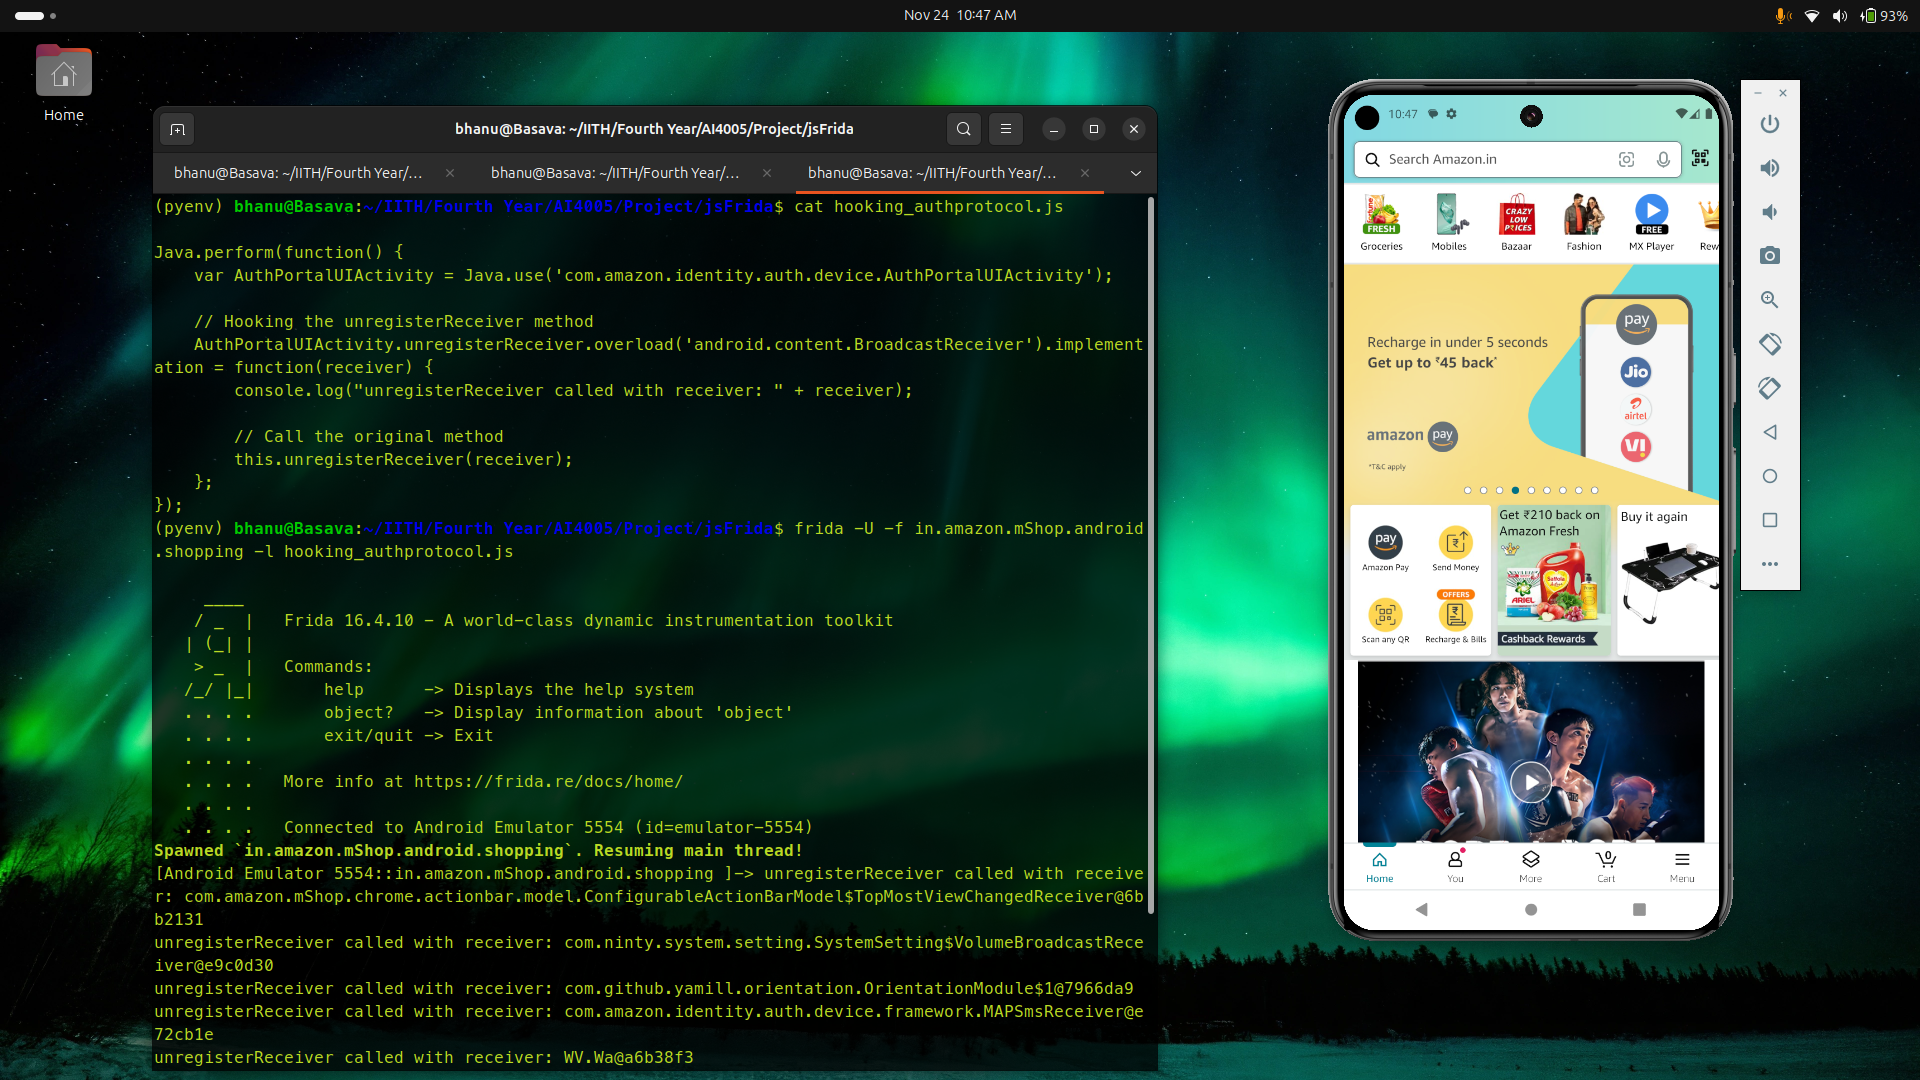
\includegraphics[width=0.9\textwidth]{../images/hooked_auth_protocol.png}
    \caption{Hooking into activity using Frida}
\end{figure}

In above image we observe 

\noindent \texttt{com.ninty.system.setting.SystemSettingsVolumeBroadcastReceiver@e9c0d30}

is the broadcater that is responsible for reading sms from the device.

Once the broadcaster is identified, we can hook into it to monitor the SMS messages being read by the application. We can then close the application and test with different SMS messages that are not OTPs. If we observe that the application reads SMS messages unrelated to OTPs, this behavior can be reported to the application developer as a potential issue.

\section{Future work}
The project has laid the foundation for further exploration of mobile application vulnerabilities related to automatic SMS reading. Future work can focus on the following areas:
\begin{itemize}
    \item Test a wider range of applications and services to identify common vulnerabilities and patterns in SMS handling.
    \item Develop Frida scripts to automate the process of monitoring and analyzing SMS interception by applications.
    \item Collaborate with mobile application developers to raise awareness of the risks associated with automatic OTP readers and implement best practices for secure SMS handling.
\end{itemize}

\section{Conclusion}  
This project successfully demonstrated the potential vulnerabilities of mobile applications that automatically read SMS messages, particularly OTPs. Through a comprehensive framework integrating a broadcaster application, Flask server, and rooted Android emulator with Frida-server, we identified critical risks in SMS handling by applications. The ability to intercept, forward, and monitor SMS data highlights the need for robust safeguards against unauthorized access and misuse. By simulating real-world scenarios, the findings emphasize the importance of stricter security measures and responsible implementation of automatic OTP readers.  

Future efforts can focus on extending this framework to other mobile security vulnerabilities, improving analysis automation, and collaborating with developers to enhance application security.  


\end{document}
